\documentclass[
%% TIKZ_CLASSOPTION %%
tikz
]{standalone}
\usepackage{amsmath}
\usetikzlibrary{matrix}
%% EXTRA_TIKZ_PREAMBLE_CODE %%
\begin{document}
%% TIKZ_CODE %%
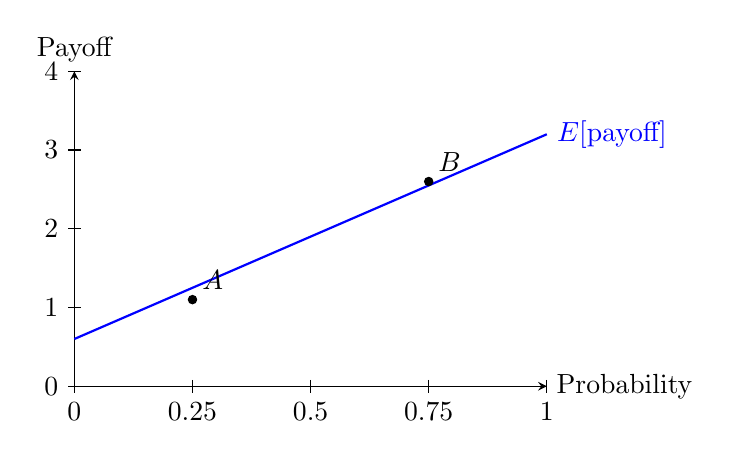
\begin{tikzpicture}[>=stealth, scale=1.0]
  % Axes
  \draw[->] (0,0) -- (6,0) node[right] {Probability};
  \draw[->] (0,0) -- (0,4) node[above] {Payoff};

  % Tick marks (x: 0 to 1)
  \foreach \x/\lab in {0/0, 1.5/0.25, 3/0.5, 4.5/0.75, 6/1}
    \draw (\x,0.08) -- (\x,-0.08) node[below] {\lab};

  % Tick marks (y)
  \foreach \y/\lab in {0/0, 1/1, 2/2, 3/3, 4/4}
    \draw (0.08,\y) -- (-0.08,\y) node[left] {\lab};

  % Example expected-payoff line
  \draw[thick, blue] (0,0.6) -- (6,3.2) node[right] {$\mathbb{E}[\text{payoff}]$};

  % Example points
  \filldraw[black] (1.5,1.1) circle (1.5pt) node[above right] {$A$};
  \filldraw[black] (4.5,2.6) circle (1.5pt) node[above right] {$B$};
\end{tikzpicture}
\end{document}
